\subsection{Le solénoïde}\label{chapter-LHC-section-CMS-subsec-solenoide}
\begin{wraptable}{R}{6.25cm}
\centering
\vspace{-\baselineskip}
\begin{tabular}{lc}
\toprule
Champ & \SI{3.8}{\tesla}\\
Diamètre interne & \SI{5.9}{\meter}\\
Longueur & \SI{12.9}{\meter}\\
Nombre de tours & \num{2168}\\
Courant & \SI{19.5}{\kilo\ampere}\\
Énergie stockée & \SI{2.7}{\giga\joule}\\
\bottomrule
\end{tabular}
\caption[Caractéristiques du solénoïde supraconducteur de CMS.]{Caractéristiques du solénoïde supraconducteur de CMS~\cite{CMS_TDR_1}.}
\label{tab-solenoid_properties}
\vspace{\baselineskip}
\end{wraptable}
Le solénoïde supraconducteur est une des parties les plus importantes du détecteur.
Il aide à caractériser les particules électriquement chargées issues des collisions.
En effet, un champ magnétique courbe les trajectoires des particules électriquement chargées.
Pour une particule d'impulsion $\vec{p}$, de charge $q$ et de vitesse $\vec{v}$ soumise à un champ magnétique $\vec{B}$,
\begin{equation}
\dv{\vec{p}}{t} = q \vec{v} \wedge \vec{B}
\mend
\end{equation}
Il s'agit de la composante magnétique de la force de Lorentz.
Avec un champ magnétique dirigé \og vers le haut \fg, une particule chargée positivement est ainsi déviée vers la droite et une particule chargée négativement vers la gauche.
Le rayon de courbure $r$ de la trajectoire de la particule est
\begin{equation}
r = \frac{\pT}{\abs{q}B}
\label{eq-chapter-LHC-section-CMS-subsec-solenoide-rayon_courbure}
\end{equation}
avec \pT\ l'impulsion dans le plan transverse au champ magnétique.
Dans le cas du détecteur CMS, le champ magnétique est aligné avec l'axe du faisceau, il s'agit donc également de l'impulsion transverse définie dans la section~\ref{chapter-LHC-section-CMS-subsec-overview_and_coordinates}.
Les particules chargées se propagent ainsi selon une trajectoire hélicoïdale autour de l'axe du faisceau et les particules neutres en ligne droite.
\par Afin d'assurer de bonnes performances sur l'identification des particules, en particulier sur la détermination du signe de la charge des muons (permettant de savoir s'il s'agit d'un muon ou d'un antimuon) et de leur impulsion jusqu'à l'ordre du \SI{}{\TeV}, la collaboration CMS a choisi d'utiliser un solénoïde supraconducteur~\cite{cms_paper,CERN-LHCC-97-010,CMS_TDR_1,CMS_magnet} dont les caractéristiques sont résumées dans le tableau~\ref{tab-solenoid_properties}.
Le rapport rayon sur longueur du cylindre défini par le solénoïde permet ainsi une identification efficace des muons de pseudo-rapidité inférieure à \num{2.4}~\cite{CERN-LHCC-97-010}.
\par À l'extérieur du solénoïde, une culasse d'acier, visible en rouge sur la figure~\ref{fig-chapter-LHC-section-CMS-subsec-overview_and_coordinates-vue_eclatee_CMS}, permet de contenir le retour du champ magnétique.
La culasse d'acier est composée de plusieurs couches séparées par les chambres à muons.
Elle présente ainsi une épaisseur cumulée d'environ \SI{1.5}{\meter}.
Le champ magnétique, au lieu d'être presque nul hors du solénoïde, atteint ainsi \num{1} à \SI{2}{\tesla} dans la culasse d'acier, selon l'endroit considéré.
Les trajectoires des muons sont alors courbées dans un sens dans le volume interne du solénoïde, puis dans l'autre sens hors du solénoïde.
La carte du champ magnétique obtenu est représentée sur la figure~\ref{fig-chapter-LHC-section-CMS-subsec-solenoide-CMS_B_field_map}.
\begin{figure}[h]
\centering
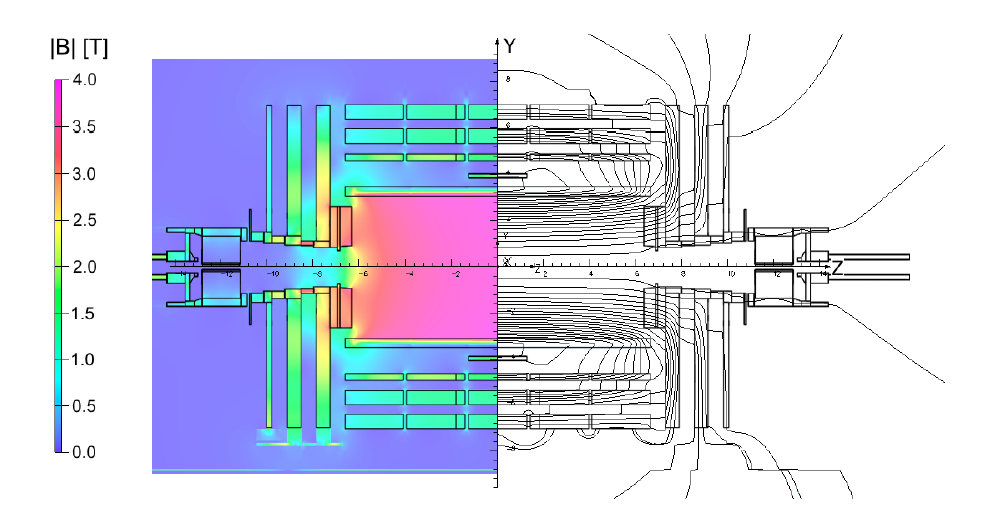
\includegraphics[width=\textwidth]{\PhDthesisdir/plots_and_images/from_CMS_magnetic_field/CMS_B_field_map.png}
\caption[Champ magnétique dans le détecteur CMS.]{Valeurs de la norme du champ magnétique (à gauche) et lignes de champ (à droite) prédites dans la section longitudinale du déteteur CMS avec une valeur du champ au centre de \SI{3.8}{\tesla}~\cite{CMS_magnetic_field}. Chaque ligne de champ correspond à un flux magnétique de \SI{6}{\weber}.}
\label{fig-chapter-LHC-section-CMS-subsec-solenoide-CMS_B_field_map}
\end{figure}